\section{Clustering} \label{sec:3.1}

\blindtext

\begin{table}[!hbt]
    \caption[Knee based Clustering with PCA]{\textbf{Knee based Clustering with PCA.}.}
    \label{tab:3.1.1}
    \pgfplotstabletypeset[
        every head row/.style={
            before row={
                \toprule
                & \multicolumn{3}{l}{\textbf{Cluster}} &  & \multicolumn{2}{l}{\textbf{mixed}} &\\
                \cmidrule(lr){2-4}\cmidrule(lr){6-7}
            },
            after row={
                \midrule
            },
        },
        every last row/.style={
            after row={
                %... & ... & ... & ... & ... & ... & ... & ...\\
                \bottomrule
            },
        },
        begin table=\begin{tabular*}{\textwidth},
        end table=\end{tabular*},
        header=false,
        skip first n=1,
        columns={0,1,2,3,4,5,6,7},
        columns/0/.style={multicolumn names=l,column name=\textbf{Segment}, column type=@{\extracolsep{\fill} }r},
        columns/1/.style={multicolumn names=l,column name=\textbf{\#Final}, column type=r},
        columns/2/.style={multicolumn names=l,column name=\textbf{\#Raw}, column type=r},
        columns/3/.style={multicolumn names=l,column name=\textbf{Normalized}, column type=r},
        columns/4/.style={multicolumn names=l,column name=\textbf{\#Unclustered}, column type=r},
        columns/5/.style={multicolumn names=l,column name=\textbf{H}, column type=r},
        columns/6/.style={multicolumn names=l,column name=\textbf{N}, column type=r},
        columns/7/.style={multicolumn names=l,column name=\textbf{Distance}, column type=r},
        %row predicate/.code={%
        %    \ifnum#1>0\relax
        %        \ifnum#1<2\relax
        %            \pgfplotstableuserowfalse
        %        \fi
        %    \fi
        %}
    ]
    {PCA/information.csv}
\end{table}

\begin{table}[!hbt]
    \caption[DBCV based Clustering with PCA]{\textbf{DBCV based Clustering with PCA.}.}
    \label{tab:3.1.2}
    \pgfplotstabletypeset[
        every head row/.style={
            before row={
                \toprule
                & \multicolumn{2}{l}{\textbf{Cluster}} &  & \multicolumn{2}{l}{\textbf{mixed}} & &\\
                \cmidrule(lr){2-3}\cmidrule(lr){5-6}
            },
            after row={
                \midrule
            },
        },
        every last row/.style={
            after row={
                %... & ... & ... & ... & ... & ... & ... & ...\\
                \bottomrule
            },
        },
        begin table=\begin{tabular*}{\textwidth},
        end table=\end{tabular*},
        header=false,
        skip first n=1,
        columns={0,1,2,3,4,5,6,7},
        columns/0/.style={multicolumn names=l,column name=\textbf{Segment}, column type=@{\extracolsep{\fill} }r},
        columns/1/.style={multicolumn names=l,column name=\textbf{\#Final}, column type=r},
        columns/2/.style={multicolumn names=l,column name=\textbf{\#Raw}, column type=r},
        columns/3/.style={multicolumn names=l,column name=\textbf{\#Unclustered}, column type=r},
        columns/4/.style={multicolumn names=l,column name=\textbf{H}, column type=r},
        columns/5/.style={multicolumn names=l,column name=\textbf{N}, column type=r},
        columns/6/.style={multicolumn names=l,column name=\textbf{Distance}, column type=r},
        columns/7/.style={multicolumn names=l,column name=\textbf{DBCV}, column type=r},
        %row predicate/.code={%
        %    \ifnum#1>0\relax
        %        \ifnum#1<2\relax
        %            \pgfplotstableuserowfalse
        %        \fi
        %    \fi
        %}
    ]
    {PCA/information_alt.csv}
\end{table}

\begin{table}[!hbt]
    \caption[Knee based Clustering with UMAP]{\textbf{Knee based Clustering with UMAP.}.}
    \label{tab:3.1.3}
    \pgfplotstabletypeset[
        every head row/.style={
            before row={
                \toprule
                & \multicolumn{3}{l}{\textbf{Cluster}} &  & \multicolumn{2}{l}{\textbf{mixed}} &\\
                \cmidrule(lr){2-4}\cmidrule(lr){6-7}
            },
            after row={
                \midrule
            },
        },
        every last row/.style={
            after row={
                %... & ... & ... & ... & ... & ... & ... & ...\\
                \bottomrule
            },
        },
        begin table=\begin{tabular*}{\textwidth},
        end table=\end{tabular*},
        header=false,
        skip first n=1,
        columns={0,1,2,3,4,5,6,7},
        columns/0/.style={multicolumn names=l,column name=\textbf{Segment}, column type=@{\extracolsep{\fill} }r},
        columns/1/.style={multicolumn names=l,column name=\textbf{\#Final}, column type=r},
        columns/2/.style={multicolumn names=l,column name=\textbf{\#Raw}, column type=r},
        columns/3/.style={multicolumn names=l,column name=\textbf{Normalized}, column type=r},
        columns/4/.style={multicolumn names=l,column name=\textbf{\#Unclustered}, column type=r},
        columns/5/.style={multicolumn names=l,column name=\textbf{H}, column type=r},
        columns/6/.style={multicolumn names=l,column name=\textbf{N}, column type=r},
        columns/7/.style={multicolumn names=l,column name=\textbf{Distance}, column type=r},
        %row predicate/.code={%
        %    \ifnum#1>0\relax
        %        \ifnum#1<2\relax
        %            \pgfplotstableuserowfalse
        %        \fi
        %    \fi
        %}
    ]
    {UMAP/information.csv}
\end{table}

\begin{table}[!hbt]
    \caption[DBCV based Clustering with PCA]{\textbf{DBCV based Clustering with PCA.}.}
    \label{tab:3.1.4}
    \pgfplotstabletypeset[
        every head row/.style={
            before row={
                \toprule
                & \multicolumn{2}{l}{\textbf{Cluster}} &  & \multicolumn{2}{l}{\textbf{mixed}} & &\\
                \cmidrule(lr){2-3}\cmidrule(lr){5-6}
            },
            after row={
                \midrule
            },
        },
        every last row/.style={
            after row={
                %... & ... & ... & ... & ... & ... & ... & ...\\
                \bottomrule
            },
        },
        begin table=\begin{tabular*}{\textwidth},
        end table=\end{tabular*},
        header=false,
        skip first n=1,
        columns={0,1,2,3,4,5,6,7},
        columns/0/.style={multicolumn names=l,column name=\textbf{Segment}, column type=@{\extracolsep{\fill} }r},
        columns/1/.style={multicolumn names=l,column name=\textbf{\#Final}, column type=r},
        columns/2/.style={multicolumn names=l,column name=\textbf{\#Raw}, column type=r},
        columns/3/.style={multicolumn names=l,column name=\textbf{\#Unclustered}, column type=r},
        columns/4/.style={multicolumn names=l,column name=\textbf{H}, column type=r},
        columns/5/.style={multicolumn names=l,column name=\textbf{N}, column type=r},
        columns/6/.style={multicolumn names=l,column name=\textbf{Distance}, column type=r},
        columns/7/.style={multicolumn names=l,column name=\textbf{DBCV}, column type=r},
        %row predicate/.code={%
        %    \ifnum#1>0\relax
        %        \ifnum#1<2\relax
        %            \pgfplotstableuserowfalse
        %        \fi
        %    \fi
        %}
    ]
    {UMAP/information_alt.csv}
\end{table}

\begin{figure}
    \begin{adjustbox}{minipage=\dimexpr\textwidth-2\fboxsep-2\fboxrule,fbox}
        \begin{subfigure}[b]{0.475\textwidth}
            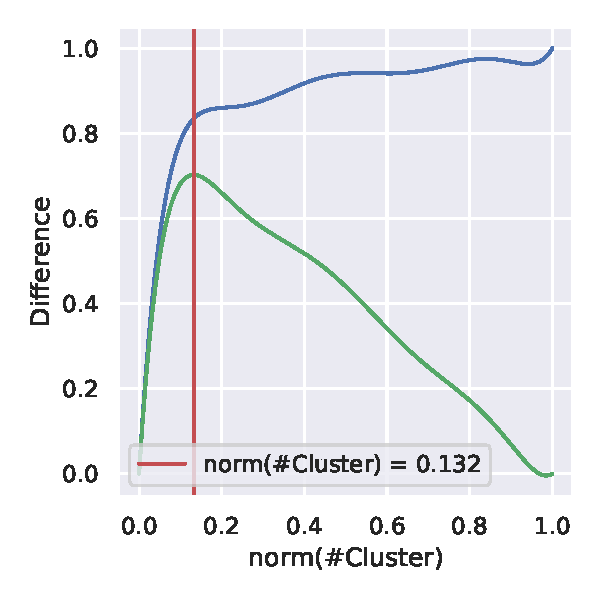
\includegraphics[width=\textwidth]{PCA/Cluster_Knee_Segment_4.pdf}
            \caption[Kneedle Algorithm]{\textbf{Kneedle Algorithm}}
            \label{fig:3.1.1a}
        \end{subfigure}
        \hfill
        \begin{subfigure}[b]{0.475\textwidth}
            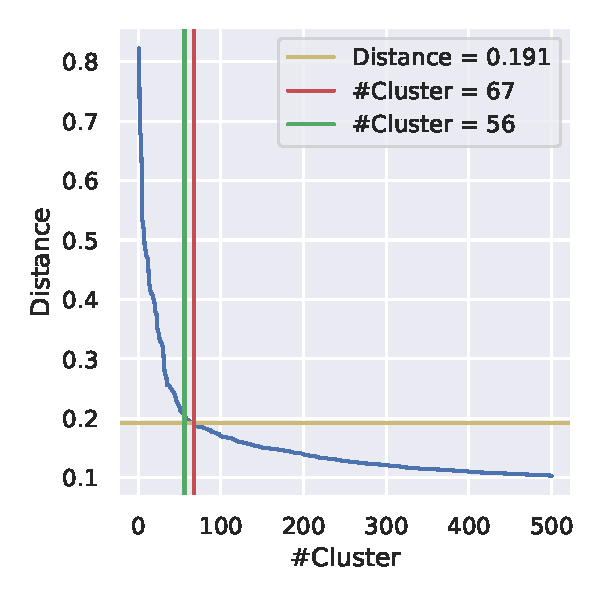
\includegraphics[width=\textwidth]{PCA/Cluster_Elbow_Knee_Segment_4.pdf}
            \caption[Kneedle Knee]{\textbf{Kneedle Knee}}
            \label{fig:3.1.1b}
        \end{subfigure}
        \vskip\baselineskip
        \begin{subfigure}[b]{0.475\textwidth}
            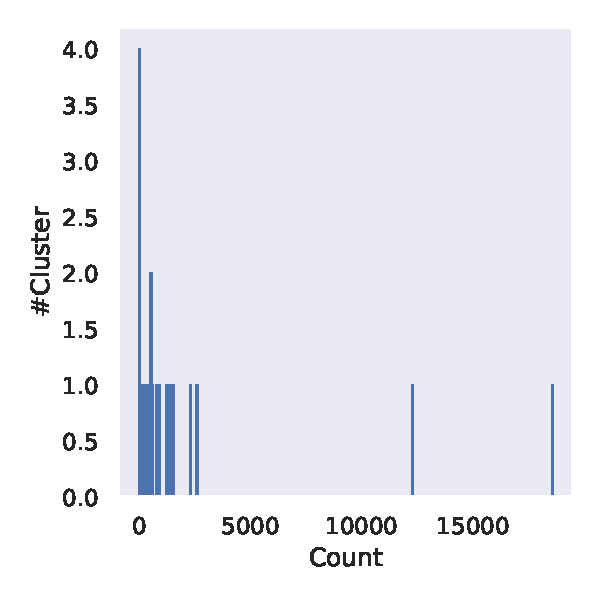
\includegraphics[width=\textwidth]{PCA/Cluster_Distribution_Segment_4.pdf}
            \caption[Cluster Distribution]{\textbf{Cluster Distribution}}
            \label{fig:3.1.1c}
        \end{subfigure}
        \hfill
        \begin{subfigure}[b]{0.475\textwidth}
            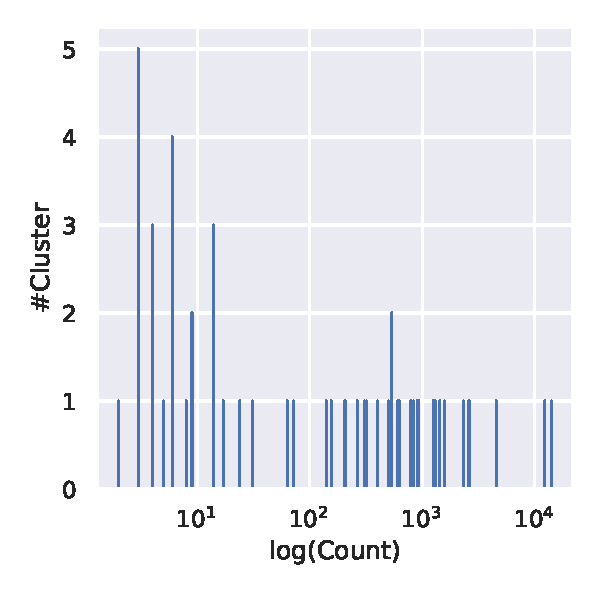
\includegraphics[width=\textwidth]{PCA/Cluster_Distribution_Log_Segment_4.pdf}
            \caption[Logarithmic Distribution]{\textbf{Logarithmic Distribution}}
            \label{fig:3.1.1d}
        \end{subfigure}
    \end{adjustbox}
    \caption[Knee based Segment 4 Clustering with PCA]{\textbf{Knee based Segment 4 Clustering with PCA.}.}
    \label{fig:3.1.1}
\end{figure}

\begin{figure}
    \begin{adjustbox}{minipage=\dimexpr\textwidth-2\fboxsep-2\fboxrule,fbox}
        \begin{subfigure}[b]{0.475\textwidth}
            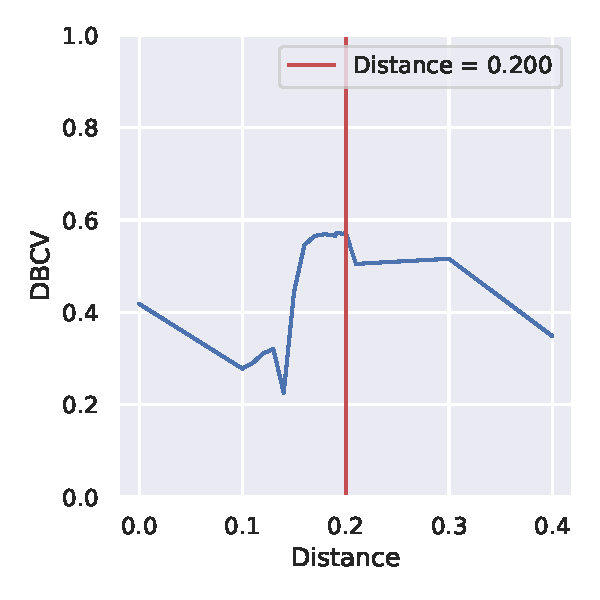
\includegraphics[width=\textwidth]{PCA/Cluster_DBCV_Segment_4.pdf}
            \caption[DBCV Exploration]{\textbf{DBCV Exploration}}
            \label{fig:3.1.2a}
        \end{subfigure}
        \hfill
        \begin{subfigure}[b]{0.475\textwidth}
            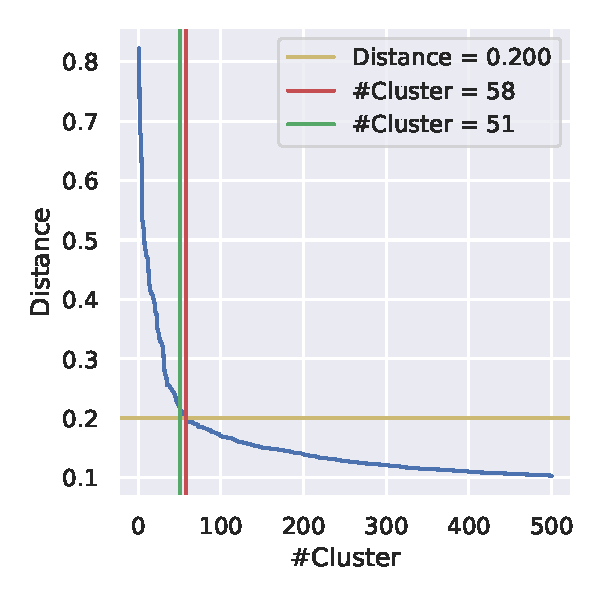
\includegraphics[width=\textwidth]{PCA/Cluster_Elbow_DBCV_Segment_4.pdf}
            \caption[DBCV Knee]{\textbf{DBCV Knee}}
            \label{fig:3.1.2b}
        \end{subfigure}
        \vskip\baselineskip
        \begin{subfigure}[b]{0.475\textwidth}
            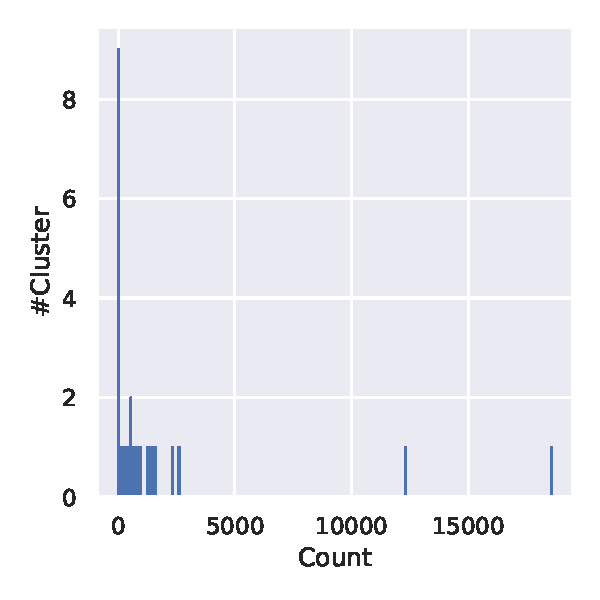
\includegraphics[width=\textwidth]{PCA/Cluster_Distribution_Segment_4_alternative.pdf}
            \caption[Cluster Distribution]{\textbf{Cluster Distribution}}
            \label{fig:3.1.2c}
        \end{subfigure}
        \hfill
        \begin{subfigure}[b]{0.475\textwidth}
            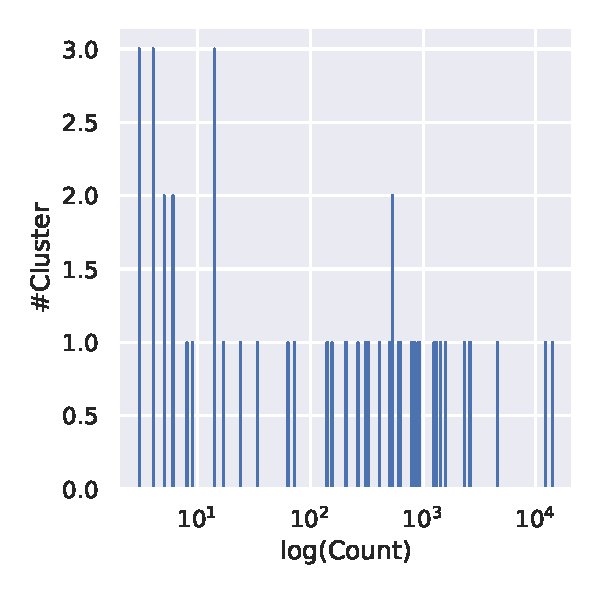
\includegraphics[width=\textwidth]{PCA/Cluster_Distribution_Log_Segment_4_alternative.pdf}
            \caption[Logarithmic Distribution]{\textbf{Logarithmic Distribution}}
            \label{fig:3.1.2d}
        \end{subfigure}
    \end{adjustbox}
    \caption[DBCV based Segment 4 Clustering with PCA]{\textbf{DBCV based Segment 4 Clustering with PCA.}.}
    \label{fig:3.1.2}
\end{figure}

\begin{figure}
    \begin{adjustbox}{minipage=\dimexpr\textwidth-2\fboxsep-2\fboxrule,fbox}
        \begin{subfigure}[b]{0.475\textwidth}
            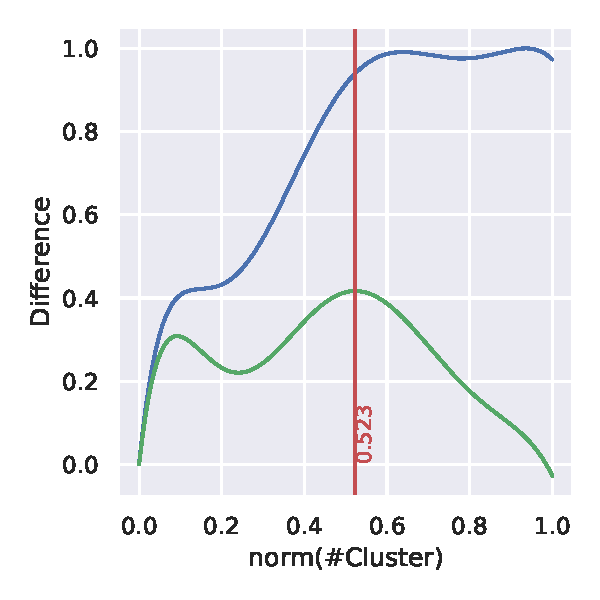
\includegraphics[width=\textwidth]{UMAP/Cluster_Knee_Segment_4.pdf}
            \caption[Kneedle Algorithm]{\textbf{Kneedle Algorithm}}
            \label{fig:3.1.3a}
        \end{subfigure}
        \hfill
        \begin{subfigure}[b]{0.475\textwidth}
            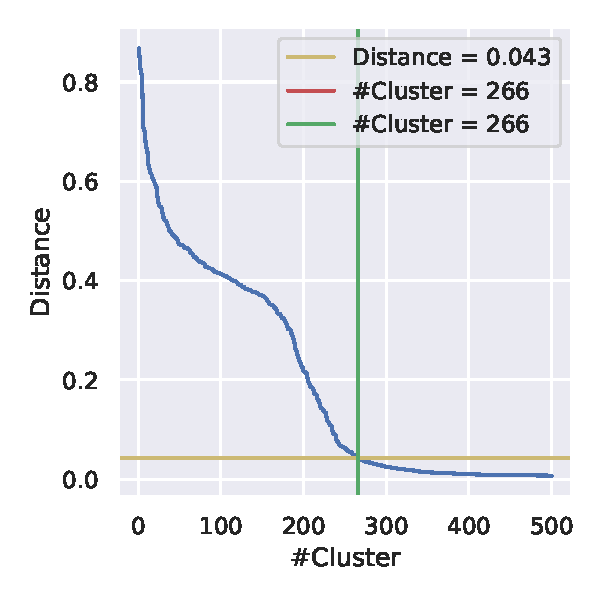
\includegraphics[width=\textwidth]{UMAP/Cluster_Elbow_Knee_Segment_4.pdf}
            \caption[Kneedle Knee]{\textbf{Kneedle Knee}}
            \label{fig:3.1.3b}
        \end{subfigure}
        \vskip\baselineskip
        \begin{subfigure}[b]{0.475\textwidth}
            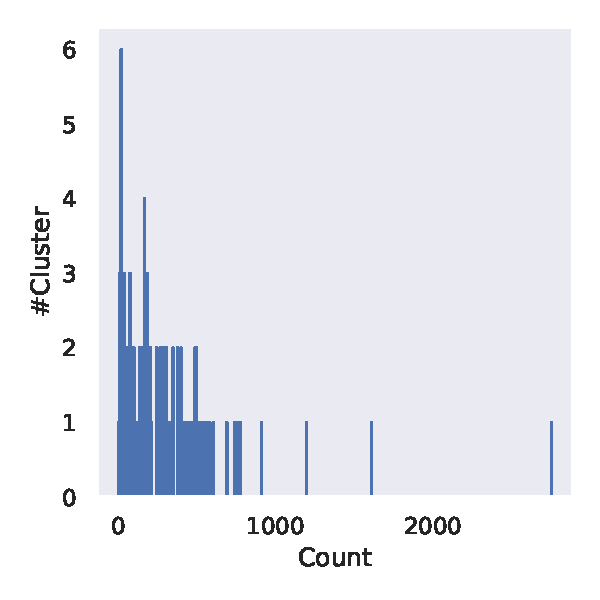
\includegraphics[width=\textwidth]{UMAP/Cluster_Distribution_Segment_4.pdf}
            \caption[Cluster Distribution]{\textbf{Cluster Distribution}}
            \label{fig:3.1.3c}
        \end{subfigure}
        \hfill
        \begin{subfigure}[b]{0.475\textwidth}
            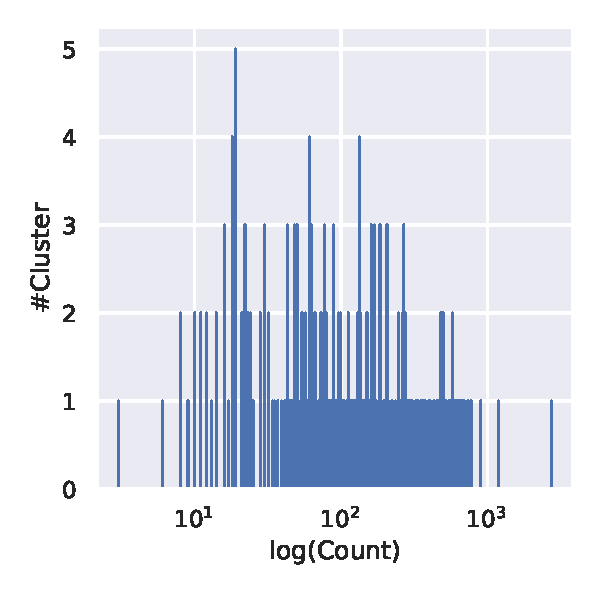
\includegraphics[width=\textwidth]{UMAP/Cluster_Distribution_Log_Segment_4.pdf}
            \caption[Logarithmic Distribution]{\textbf{Logarithmic Distribution}}
            \label{fig:3.1.3d}
        \end{subfigure}
    \end{adjustbox}
    \caption[Knee based Segment 4 Clustering with UMAP]{\textbf{Knee based Segment 4 Clustering with UMAP.}.}
    \label{fig:3.1.3}
\end{figure}

\begin{figure}
    \begin{adjustbox}{minipage=\dimexpr\textwidth-2\fboxsep-2\fboxrule,fbox}
        \begin{subfigure}[b]{0.475\textwidth}
            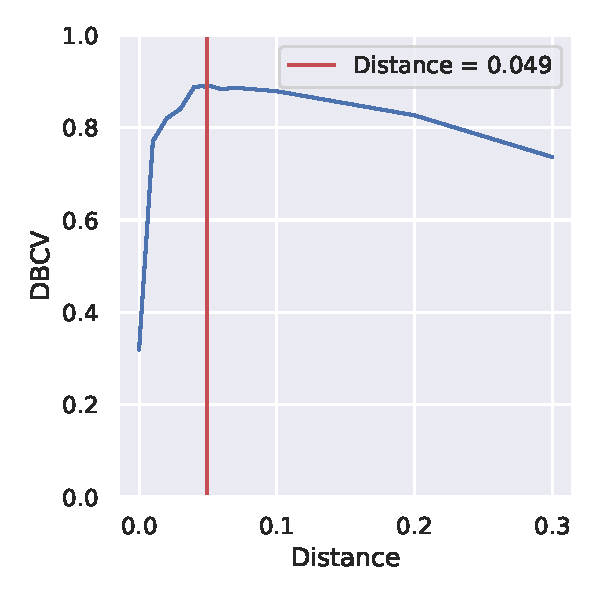
\includegraphics[width=\textwidth]{UMAP/Cluster_DBCV_Segment_4.pdf}
            \caption[DBCV Exploration]{\textbf{DBCV Exploration}}
            \label{fig:3.1.4a}
        \end{subfigure}
        \hfill
        \begin{subfigure}[b]{0.475\textwidth}
            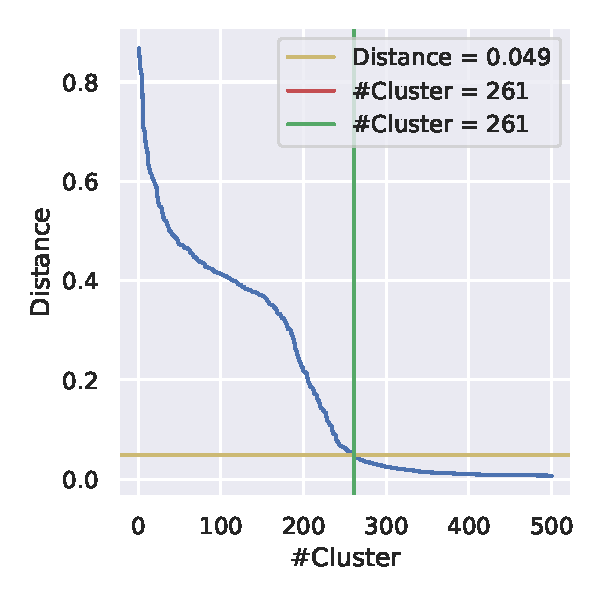
\includegraphics[width=\textwidth]{UMAP/Cluster_Elbow_DBCV_Segment_4.pdf}
            \caption[DBCV Knee]{\textbf{DBCV Knee}}
            \label{fig:3.1.4b}
        \end{subfigure}
        \vskip\baselineskip
        \begin{subfigure}[b]{0.475\textwidth}
            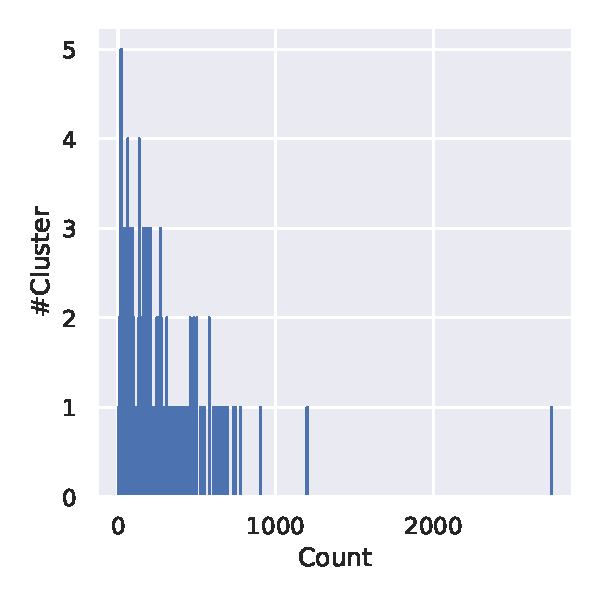
\includegraphics[width=\textwidth]{UMAP/Cluster_Distribution_Segment_4_alternative.pdf}
            \caption[Cluster Distribution]{\textbf{Cluster Distribution}}
            \label{fig:3.1.4c}
        \end{subfigure}
        \hfill
        \begin{subfigure}[b]{0.475\textwidth}
            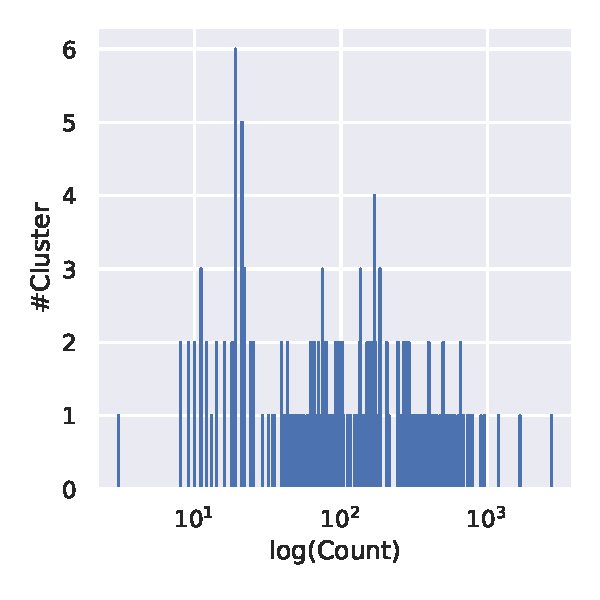
\includegraphics[width=\textwidth]{UMAP/Cluster_Distribution_Log_Segment_4_alternative.pdf}
            \caption[Logarithmic Distribution]{\textbf{Logarithmic Distribution}}
            \label{fig:3.1.4d}
        \end{subfigure}
    \end{adjustbox}
    \caption[DBCV based Segment 4 Clustering with UMAP]{\textbf{DBCV based Segment 4 Clustering with UMAP.}.}
    \label{fig:3.1.4}
\end{figure}

\begin{table}[!hbt]
    \caption[Knee based Clustering with PCA]{\textbf{Knee based Clustering with PCA.}.}
    \label{tab:3.1.5}
    \pgfplotstabletypeset[
        every head row/.style={
            before row={
                \toprule
            },
            after row={
                \midrule
            },
        },
        every last row/.style={
            after row={
                ... & ... & ... & ... & ... & ... & ... & ...\\
                \bottomrule
            },
        },
        begin table=\begin{tabular*}{\textwidth},
        end table=\end{tabular*},
        header=false,
        skip first n=1,
        columns={0,1,2,3,4,5,6},
        columns/0/.style={multicolumn names=l,column name=\textbf{Accession}, column type=@{\extracolsep{\fill} }r},
        columns/1/.style={multicolumn names=l,column name=\textbf{Segment}, column type=r},
        columns/2/.style={multicolumn names=l,column name=\textbf{Cluster}, column type=r},
        columns/3/.style={multicolumn names=l,column name=\textbf{H}, column type=r},
        columns/4/.style={multicolumn names=l,column name=\textbf{Centroid}, column type=r},
        columns/5/.style={multicolumn names=l,column name=\textbf{N}, column type=r},
        columns/6/.style={multicolumn names=l,column name=\textbf{Strain}, column type=r},
    ]
    {PCA/cluster_head.csv}
\end{table}

\blindtext